\documentclass[12 pt]{extarticle}

	\usepackage[frenchb]{babel}
	\usepackage[utf8]{inputenc}  
	\usepackage[T1]{fontenc}
	\usepackage{amssymb}
	\usepackage[mathscr]{euscript}
	\usepackage{stmaryrd}
	\usepackage{amsmath}
	\usepackage{tikz}
	\usepackage[all,cmtip]{xy}
	\usepackage{amsthm}
	\usepackage{varioref}
	\usepackage{pstricks-add, pst-plot}
\usepackage{auto-pst-pdf}
	\usepackage[margin=0.55in]{geometry}
	\geometry{a4paper}
	\usepackage{lmodern}
	\usepackage{hyperref}
	\usepackage{array}
	 \usepackage{fancyhdr}
	 \usepackage{float}
	\pagestyle{fancy}
	\theoremstyle{plain}
	\fancyhead[L]{Contrôle}
	\fancyfoot[C]{\emph{Sujet recto-verso}}
	\fancyhead[R]{10 novembre 2025}

	\title{Interrogation de calcul}
	\date{}
	\begin{document}

\begin{center}{\Large Contrôle de calcul littéral}\\
\emph{Toute réponse devra être rédigée sur une copie double dûment présentée. La calculatrice est interdite. L'ordre des exercices est libre.} 
 \end{center} 
 \subsection*{Exercice 1 (8 points)}
   \begin{enumerate}
   \item Réduire : $(-3x)^3$
   \item Réduire : $4-(8a+15)$
   \item Réduire : $-(8y-15)-1$
   \item Réduire : $(2x-4)-(x+2)$
   \item Développer et réduire : $(9x-2)(-3x+5)$
   \item Factoriser $10x- 4xy + 2xz$.
   \item Factoriser $3(2x+6) + (x+1)(2x+6)$
   \item Factoriser $(3x+4)(x+1) - (2x-2)(3x+4)$
    \end{enumerate}


 \subsection*{Exercice 2- DNB Polynésie 2025 (1,5+1,5+3= 6 points)}  
 \begin{center}
 
\includegraphics[scale=.9]{Exo2}\end{center}
 
 \newpage
 \subsection*{Exercice 3 - DNB Métropole 2024  (1+1+1+1,5+1,5=6 points)}

On considère les deux programmes de calcul suivants :
\begin{center}
 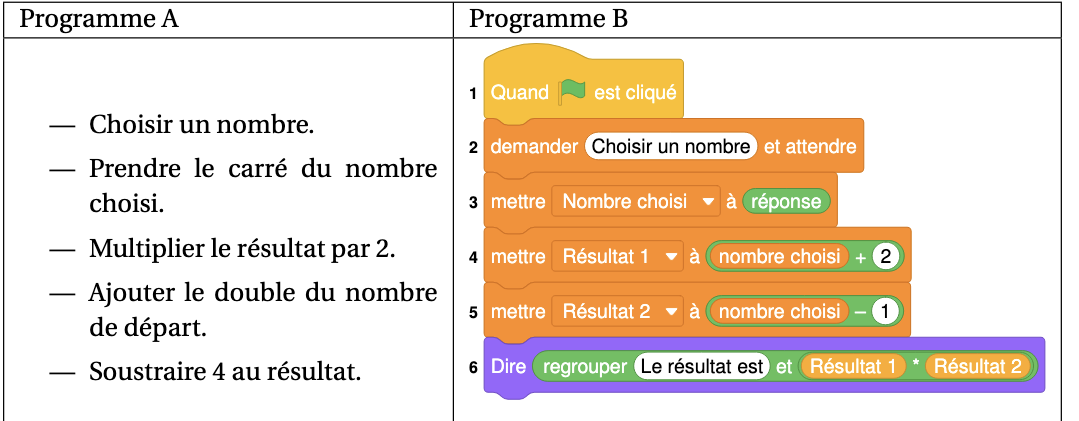
\includegraphics[scale=.8]{Programme}

\end{center}
\begin{enumerate}
\item 
	\begin{enumerate}
		\item Si on choisit le nombre $5$, vérifier qu'on obtient 56 à la fin du programme A.
		\item Si on choisit le nombre $- 9$, quel résultat obtient-on à la fin du programme B ?
	\end{enumerate}	
\item On note $x$ le nombre choisi au départ
	\begin{enumerate}
		\item Parmi les trois expressions suivantes, laquelle décrit le résultat du programme B ? 
		\[ E_1 = (x+2) - 1 \phantom{miaouaou}E_2=(x+2)\times(x-1)
		\phantom{miaouaou}x+2\times x -1\]
		\item Exprimer en fonction de $x$ le résultat obtenu avec le 
		programme $A$.
	\end{enumerate}
	\item Démontrer que le résultat du programme $B$ est toujours le double de celui du programme $A$. 
\end{enumerate}

\subsection*{Bonus}
Développer et réduire : \[(4a+5b)(6a-2b)-(4a-1)(6a+2b)-(2a-2b)(5b-1)\]
 	\end{document}
